\documentclass[conference]{IEEEtran}

\usepackage{amsmath,amssymb,amsfonts}
\usepackage{booktabs}
\usepackage{graphicx}
\usepackage{multirow}
\usepackage{url}
\usepackage{xcolor}

\graphicspath{{figures/}}

\newcommand{\CertiCut}{\textsc{CertiCut}}
\newcommand{\OPT}{\mathrm{OPT}}
\newcommand{\LB}{\mathrm{LB}}
\newcommand{\UB}{\mathrm{UB}}
\newcommand{\gap}{\Delta}

\title{CertiCut: Capacitated K-Way Independent-QPD Circuit Cutting with Anytime Overhead Bounds}

\author{\IEEEauthorblockN{Phung Trong Hung}
\IEEEauthorblockA{\textit{Faculty of Information Technology}\\
HUTECH University\\
phungtronghung0808@gmail.com}}

\begin{document}
\maketitle

% ===================================================================
% ABSTRACT
% ===================================================================
\begin{abstract}
Circuit cutting trades quantum-device width for a quasiprobability sampling overhead that can grow multiplicatively with severed interactions. We formulate static capacitated $K$-way logical-qubit partitioning with gate cuts under a fixed independent per-gate quasiprobability-decomposition (QPD) model. Aggregating gate occurrences by interaction pair in the log domain yields a weighted capacitated graph-partitioning MIP. For any $K\geq2$, any feasible capacity bounds, and any valid global bounds $\LB\leq\OPT\leq\UB$, an incumbent obeys $\Gamma_{\mathrm{inc}}/\Gamma^*\leq\exp(\UB-\LB)$. On a replicated 144-run heterogeneous matrix through $n=60$ and $K=5$, 101/144 runs reach solver-tolerance closure within 10~s; open cases retain explicit finite factors. A capacity-exact weighted K-way greedy-swap baseline returns feasible partitions for all records in milliseconds, and SCIP bounds quantify its overhead regret on closed instances. A separate 36-instance algorithm-derived matrix exposes the same K-way boundary. We also show objective reversals where minimizing cut count does not minimize independent-QPD overhead. All empirical bounds are solver-tolerance quantities, not independently verified numerical proofs.
\end{abstract}

\begin{IEEEkeywords}
quantum circuit cutting, quasiprobability decomposition, capacitated graph partitioning, anytime optimization, mixed-integer programming
\end{IEEEkeywords}

% ===================================================================
% I. INTRODUCTION
% ===================================================================
\section{Introduction}

Near-term quantum processors remain limited in qubit count, fidelity, and connectivity~\cite{preskill2018}. Circuit cutting mitigates the width constraint by decomposing a circuit into smaller, independently executable fragments and recovering the target quantity through classical post-processing~\cite{peng2020,bravyi2016,tang2021}. This tradeoff can be expensive: every severed interaction contributes a gate-dependent quasiprobability sampling factor, and these factors multiply across cuts. Minimizing the number of cuts therefore need not minimize the resulting sampling overhead.

Automatic cutting workflows commonly report a partition and a solver-specific status. Although generic mixed-integer programming (MIP) solvers expose primal and dual bounds, their implications for circuit-cutting resource overhead are not explicit in the solver output. Such a translation matters because an additive objective gap can represent orders of magnitude in multiplicative sampling cost. Working in the log-overhead domain makes the connection exact: a global optimization gap immediately yields a worst-case overhead ratio.

We present \CertiCut{}, a solver-independent resource-semantics framework and a capacitated $K$-way independent-QPD MIP. The formulation targets logical interaction graphs, supports arbitrary declared fragment counts and per-fragment lower/upper capacities, and uses independent gate-level QPD costs from Qiskit Addon Cutting~0.10~\cite{qiskitcutting}. In exact arithmetic, global bounds at a safe stopping boundary imply $F=\exp(\UB-\LB)$; runtime outputs are floating-point solver-tolerance quantities. The production optimizer is SCIP. A specialized B2S branch-and-bound implementation remains a $K=2$ balanced-bisection reference for polyhedral ablation, not a production-performance claim.

\begin{figure}[t]
  \centering
  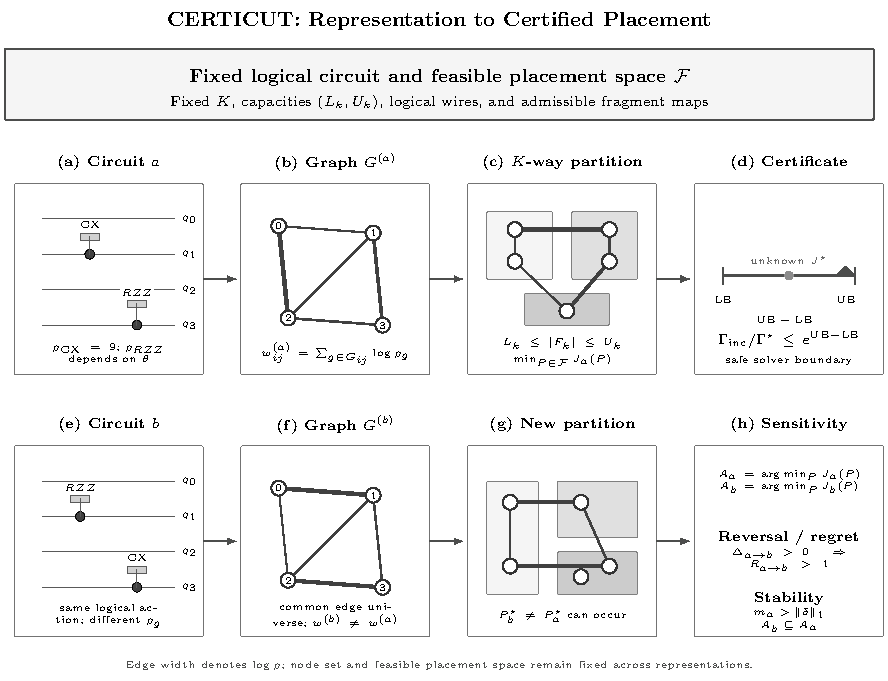
\includegraphics[width=\columnwidth]{fig_certicut_architecture.pdf}
  \caption{\CertiCut{} workflow. The independent-QPD model reduces to capacitated $K$-way graph partitioning. SCIP supplies solver-tolerance primal/dual bounds, interpreted through $F=\exp(\UB-\LB)$. The $K=2$ B2S reference supports polyhedral ablation.}
  \label{fig:architecture}
\end{figure}

This work makes three contributions:
\begin{enumerate}
  \item \textbf{Capacitated $K$-way formulation and model-overhead semantics.} For arbitrary $K\geq2$, lower/upper fragment capacities, fixed representation, and independent per-gate QPD, we give an exact assignment/locality MIP. In exact arithmetic, a global gap gives $\Gamma_{\mathrm{inc}}/\Gamma^*\leq\exp(\UB-\LB)$; implementation outputs are labelled solver-tolerance bounds.

  \item \textbf{Structural and empirical consequences.} We characterize fixed-capacity cross-pair cardinality, retain a $K=2$ B2S strengthening study, show count-versus-QPD objective reversals, and evaluate heterogeneous $K\in\{2,3,4,5\}$ scaling through $n=60$ with three seeds per cell. The 144-run matrix reports both closure and open-case factors rather than hiding computational boundaries.

  \item \textbf{Transparent scope and backend boundary.} The evaluation fixes the independent-QPD model and reports closure together with finite open-case factors. Basic SCIP is the strongest evaluated production backend; no custom-solver superiority claim is made.
\end{enumerate}

The remainder develops the formulation and bound semantics, then evaluates objective reversals and $K$-way backend behavior. Throughout, we separate circuit-cutting model semantics from optimization-backend performance.

% ===================================================================
% II. BACKGROUND AND PROBLEM FORMULATION
% ===================================================================
\section{Background and Problem Formulation}

\subsection{Independent QPD Circuit Cutting}

Gate cutting replaces selected two-qubit channels by quasiprobability decompositions (QPDs) over fragment-local channels~\cite{peng2020,mitarai2021}. For a cuttable channel $\mathcal{U}_g=\sum_i a_{g,i}\mathcal{E}_{g,i}$, the corresponding independent sampling overhead is
\begin{equation}
  \rho_g = \left(\sum_i |a_{g,i}|\right)^{\!2}.
  \label{eq:gate-overhead}
\end{equation}
For a partition $P$ with crossed-gate set $S(P)$, independent sampling across gates gives
\begin{equation}
  \Gamma(P) = \prod_{g \in S(P)} \rho_g, \qquad
  J(P) = \log \Gamma(P) = \sum_{g \in S(P)} \log \rho_g.
  \label{eq:objective}
\end{equation}
This objective matches the independent gate-level model in Qiskit Addon Cutting~0.10~\cite{qiskitcutting}; it is not a model of joint decompositions, finite-shot variance, or hardware noise. Because the QPD coefficient one-norm is at least one, $\rho_g\geq1$ and all log weights are nonnegative. We validated the gate costs against the Qiskit QPD registry: $\rho_{\mathrm{CX}}=\rho_{\mathrm{CZ}}=9$, $\rho_{\mathrm{iSWAP}}=\rho_{\mathrm{DCX}}=49$, $\rho_{\mathrm{CS}}=3+2\sqrt{2}\approx5.828$, and $\rho_{RZZ(\theta)}=(1+2|\sin\theta|)^2$ for numerically bound rotations.

\subsection{Log-Domain Interaction Graph}

Let $V=\{0,\ldots,n{-}1\}$ be the circuit qubits, and let $G_{ij}$ contain the two-qubit gate occurrences acting on pair $(i,j)$. We assign the nonnegative interaction weight
\begin{equation}
  w_{ij} = \sum_{g \in G_{ij}} \log \rho_g.
  \label{eq:weight}
\end{equation}
For any fragment map $f:V\rightarrow\{1,\ldots,K\}$, the objective becomes
\begin{equation}
  J(P) = \sum_{i < j} w_{ij}\,\mathbf{1}[f(i)\neq f(j)].
  \label{eq:graph-objective}
\end{equation}
The binary bisection identity $\mathbf{1}[f(i)\neq f(j)]=|z_i-z_j|$ is recovered when $K=2$.

\textbf{Proposition~1} (Objective equivalence). \textit{Under independent gate-level QPD, minimizing~\eqref{eq:objective} is equivalent to minimizing~\eqref{eq:graph-objective}.}

\emph{Proof.} Every $g\in G_{ij}$ is cut exactly when $f(i)\neq f(j)$. Regrouping the gate-level sum by qubit pair yields~\eqref{eq:graph-objective}. \hfill$\square$

\subsection{Capacitated $K$-Way Partition Problem}

Let $K\geq2$ be the declared fragment count. Binary assignment $a_{ik}=1$ denotes that qubit $i$ belongs to fragment $k$, with capacities $L_k\leq\sum_i a_{ik}\leq U_k$. For each aggregated interaction edge $e=(i,j)$, locality variable $y_{ek}=1$ denotes that both endpoints occupy fragment $k$, while $z_e=1$ denotes a crossed interaction. The exact independent-QPD MIP is
\begin{equation}
\begin{aligned}
\min\quad & \sum_{e\in E} w_e z_e\\
\text{s.t.}\quad & \sum_{k=1}^{K} a_{ik}=1 && \forall i,\\
& L_k\leq\sum_i a_{ik}\leq U_k && \forall k,\\
& y_{ek}\leq a_{ik},\quad y_{ek}\leq a_{jk} && \forall e=(i,j),k,\\
& y_{ek}\geq a_{ik}+a_{jk}-1 && \forall e=(i,j),k,\\
& z_e+\sum_{k=1}^{K}y_{ek}=1 && \forall e,\\
& a_{ik},y_{ek},z_e\in\{0,1\}.&
\end{aligned}
\label{eq:kway}
\end{equation}
The three inequalities are the exact binary AND hull. Since each endpoint has exactly one assignment, exactly one $y_{ek}$ is one iff both endpoints share a fragment; otherwise all locality variables are zero and $z_e=1$. Thus~\eqref{eq:kway} exactly optimizes~\eqref{eq:graph-objective} for arbitrary feasible capacities.

\textbf{Proposition~2} (Objective equivalence for capacitated $K$-way partitioning). \textit{For any $K\geq2$ and feasible capacities, the objective of~\eqref{eq:kway} equals the independent gate-level log overhead~\eqref{eq:objective}.}

\emph{Proof.} The assignment/locality constraints set $z_e=1$ exactly when endpoints of aggregate edge $e$ are in different fragments. Equation~\eqref{eq:weight} sums the log overhead of every gate occurrence in $G_e$. Regrouping~\eqref{eq:objective} by edge yields $\sum_e w_ez_e$. \hfill$\square$

Problem~\eqref{eq:kway} is NP-hard because exact-balanced weighted bisection is its $K=2$ special case.

\subsection{Fixed-Capacity Cardinality and the Balanced $K\!=\!2$ Special Case}

If fragment sizes are fixed exactly as $|F_k|=n_k$, every feasible partition crosses
\begin{equation}
  \sum_{i<j}\mathbf{1}[f(i)\neq f(j)]
  = \binom{n}{2}-\sum_{k=1}^{K}\binom{n_k}{2}
  = \frac12\left(n^2-\sum_{k=1}^{K}n_k^2\right)
  \label{eq:kway-cardinality}
\end{equation}
complete-graph pairs. This is a structural identity, not a constraint for lower/upper-only capacities. Exact-balanced bisection is the special case $K=2$, $n_1=n_2=n/2$, yielding $n^2/4$.

\textbf{Proposition~3} (Trivial sparse root relaxation). \textit{For exact capacities $L_k=U_k=n_k$, the LP relaxation of the sparse edge-only formulation~\eqref{eq:kway} has objective zero.}

\emph{Proof.} Set $a_{ik}=n_k/n$ and $y_{ek}=n_k/n$ for every qubit $i$, edge $e$, and fragment $k$, then set $z_e=0$. Assignment and capacity equalities hold since $\sum_kn_k=n$. The upper AND inequalities hold at equality; the lower inequality holds because $n_k/n\geq2n_k/n-1$. Finally, $z_e+\sum_ky_{ek}=1$. Thus this is LP feasible with zero nonnegative objective. \hfill$\square$

We therefore tested an all-pair extension of~\eqref{eq:kway} that imposes~\eqref{eq:kway-cardinality} with auxiliary nonedge variables, complete-metric triangles, and $a_{0,1}=1$ for equal capacities. The extension is valid but dense. On a 36-record $n\in\{20,32\}$ ablation at 5~s, the base formulation closes 31 records, symmetry-only closes 29, and the cardinality or cardinality-plus-metric variants close 6 each. Thus production E9 uses SCIP's sparse assignment/locality formulation with the valid equal-capacity anchor only; the anchor removes only a subset of label symmetry, and stronger symmetry handling remains future work because it showed no end-to-end gain in this ablation.

\subsection{Exact Balanced $K\!=\!2$ Reference Problem}

The specialized reference implementation uses the $K=2$ exact-balanced special case. All legacy reference circuits have even $n$; it requires $n/2$ qubits per fragment and fixes $z_0=0$ to remove label symmetry:
\begin{equation}
  \min_{z \in \{0,1\}^n} \sum_{i<j} w_{ij}\,|z_i - z_j|
  \quad \text{s.t.} \quad \textstyle\sum_i z_i = n/2,\; z_0 = 0.
  \label{eq:balanced}
\end{equation}
Every feasible bisection cuts exactly $(n/2)^2$ pairs in the complete-pair representation:
\begin{equation}
  \sum_{i<j} x_{ij} = n^2/4.
  \label{eq:cardinality}
\end{equation}
This identity is central to the strengthened relaxation below.

% ===================================================================
% III. THE CERTICUT OPTIMIZER
% ===================================================================
\section{Optimization Formulations and Bound Semantics}

\subsection{Exact MILP Validation Oracle}

We use a compact MIP and brute-force enumeration as independent validation oracles. For one pair $(i,j)$, the convex hull of $x_{ij}=|z_i-z_j|$ is described by
\begin{equation}
\begin{aligned}
  x_{ij} &\geq z_i-z_j, & x_{ij} &\geq z_j-z_i,\\
  x_{ij} &\leq z_i+z_j, & x_{ij} &\leq 2-z_i-z_j.
\end{aligned}
  \label{eq:xor}
\end{equation}
The implementation uses an equivalent one-hot assignment model. Its MIP retains only the two lower inequalities in~\eqref{eq:xor} and declares $x_{ij}$ binary; for positive-weight interacting pairs, minimization sets $x_{ij}$ to its exact XOR value. Zero-weight pairs do not affect the objective. SciPy/HiGHS solves this MIP, while exhaustive enumeration supplies a second oracle through 16 qubits. Neither oracle contributes bounds to the anytime results.

\subsection{Basic Assignment Relaxation}

The basic reference LP, denoted A0, uses one-hot assignment variables on qubits and cut variables only for interacting pairs. It retains exact balance and the two lower XOR inequalities from~\eqref{eq:xor}, then relaxes all variables to $[0,1]$. Because the weights are nonnegative, this is a valid lower relaxation. It is nevertheless weak: fractional assignments can make many weighted cut variables small simultaneously.

\subsection{B2S Polyhedral Strengthening}

B2S lifts A0 to the complete pair space, imposes the full XOR hull~\eqref{eq:xor}, and adds two families of valid constraints. To isolate the added families independently of this representation change, Sec.~V compares them against a complete-pair baseline, denoted CP0.

\textit{Balanced-cut cardinality.} Equality~\eqref{eq:cardinality} fixes the total cut mass over all qubit pairs.

\textit{Metric inequalities.} For each triple $(i,j,k)$, the cut polytope satisfies~\cite{deza1997}
\begin{align}
  x_{ij} - x_{ik} - x_{jk} &\leq 0, \label{eq:tri1}\\
  x_{ik} - x_{ij} - x_{jk} &\leq 0, \label{eq:tri2}\\
  x_{jk} - x_{ij} - x_{ik} &\leq 0, \label{eq:tri3}\\
  x_{ij} + x_{ik} + x_{jk} &\leq 2. \label{eq:tri4}
\end{align}
Among three binary labels, the number of pairwise disagreements is zero or two; inequalities~\eqref{eq:tri1}--\eqref{eq:tri4} exclude the fractional analogues of one or three disagreements. B2S solves the root LP, separates violated inequalities, and repeats until no violation remains or the separation budget is exhausted. The resulting pool is then reused throughout the search tree; no node-level separation is performed.

\textbf{Proposition~4} (Objective-bound redundancy without cardinality). \textit{For nonnegative weights, adding~\eqref{eq:tri1}--\eqref{eq:tri4} to CP0 does not change its optimal value. This is an objective statement, not a claim that the metric inequalities leave the CP0 polyhedron unchanged.}

\emph{Proof.} Take an optimal CP0 solution and retain its label vector $z$. Set $x_{ij}=|z_i-z_j|$ for every pair. This extension satisfies the pairwise XOR hull and all metric inequalities because absolute distance on the line is a metric and, for $z_i\in[0,1]$, $|z_i-z_j|+|z_i-z_k|+|z_j-z_k|\leq2$. For fixed $z$, these are the smallest feasible pair values; nonnegative weights therefore ensure that the objective does not increase. Hence the metric-augmented optimum is no larger than the CP0 optimum. The reverse inequality follows because constraints were added. \hfill$\square$

\textbf{Proposition~5} (Relaxation validity). \textit{The B2S LP optimum is a valid lower bound on the $K=2$ reference $\OPT$.}

\emph{Proof.} For binary labels, $x_{ij}=|z_i-z_j|$ satisfies~\eqref{eq:xor}. A balanced partition cuts $|F_0||F_1|=n^2/4$ complete-graph pairs, and each label triple satisfies~\eqref{eq:tri1}--\eqref{eq:tri4}. Hence every feasible integral bisection remains feasible in the relaxation, whose minimum cannot exceed $\OPT$. \hfill$\square$

\subsection{CertiCut Reference Implementation}

H2 constructs feasible bisections from deterministic degree-based orderings and a spectral initialization based on the graph Laplacian's Fiedler vector. Each candidate undergoes best-improving Kernighan--Lin-style swaps between fragments until no improving swap remains. The best candidate initializes $\UB$; H2 does not establish a lower bound or certify optimality.

\subsection{Backend-Independent Gap Semantics}

\textbf{Theorem~1} (Gap-to-overhead translation, exact arithmetic). \textit{For any $K\geq2$, feasible capacity bounds, and optimization backend, if $\LB\leq\OPT\leq\UB$, where $\UB=J(P_{\mathrm{inc}})$ for a feasible incumbent of~\eqref{eq:kway}, then}
\begin{equation}
  \frac{\Gamma(P_{\mathrm{inc}})}{\Gamma^*}
  = \exp(\UB-\OPT) \leq \exp(\UB-\LB).
  \label{eq:gap-translation}
\end{equation}

\emph{Proof.} Equation~\eqref{eq:objective} gives $\Gamma(P)=\exp(J(P))$. Since $\OPT\geq\LB$, exponentiation yields~\eqref{eq:gap-translation}. \hfill$\square$

This result depends on the specified independent-QPD objective and valid global bounds, not on how a backend obtains them. Proposition~6 below establishes the required bound premise for the $K=2$ \CertiCut{} reference search in exact arithmetic.

\subsection{Reference Branch-and-Bound}

The reference optimizer maintains open nodes in nondecreasing order of their LP bounds. It expands the best-bound node, updates the incumbent when an integral solution improves $\UB$, and otherwise branches on the most fractional label. Child LPs reuse the root cut pool; any child whose lower bound is at least $\UB$ is pruned. After all LP solves associated with an expansion have completed, the algorithm reaches a \emph{safe boundary} and computes
\begin{equation}
  \LB = \min\!\left(\UB,\; \min_{N \in \mathcal{F}} \LB_N\right),
  \label{eq:global-lb}
\end{equation}
where $\mathcal{F}$ denotes the open frontier. The additive log-domain gap and the corresponding multiplicative overhead factor are
\begin{equation}
  \gap = \UB - \LB, \qquad F = \exp(\gap).
  \label{eq:factor}
\end{equation}

\textbf{Proposition~6} (Reference safe-boundary validity, exact arithmetic). \textit{In exact arithmetic, every reference-search safe stopping boundary satisfies $\LB\leq\OPT\leq\UB$.}

\emph{Proof.} Feasibility of the incumbent gives $\OPT\leq\UB$. Every unexplored feasible solution belongs to a frontier subtree whose LP value lower-bounds all integral completions in that subtree. Equation~\eqref{eq:global-lb} therefore gives $\LB\leq\OPT$. \hfill$\square$

Experimental deadlines are \emph{soft}: the reference optimizer stops only at a safe boundary. We report the actual boundary time and never assign a later bound report to an earlier checkpoint. Propositions~5--6 are exact-arithmetic statements. Runtime results use floating-point HiGHS or SCIP bounds and are therefore labelled solver-tolerance quantities, not independently verified numerical proofs. A formal numerical bound would additionally require a verified conservative lower-bound procedure, such as dual-feasible recovery with outward rounding or rational/interval verification.

\begin{figure}[t]
\centering
\fbox{\begin{minipage}{0.94\columnwidth}
\small
\textbf{Algorithm: Anytime CertiCut Reference Search}\medskip\\
\textbf{Input:} QPD-weighted interaction graph $G$, capacity $q_{\max} = n/2$, soft deadline $T$.\smallskip\\
\textbf{Step 1.} Compute initial feasible partition and upper bound: $(P_{\mathrm{inc}}, \UB) \leftarrow \textsc{H2}(G)$.\smallskip\\
\textbf{Step 2.} Solve and strengthen root LP via B2S separation: $(\LB_0, \mathcal{C}) \leftarrow \textsc{B2S\text{-}Root}(G)$. Freeze cut pool~$\mathcal{C}$.\smallskip\\
\textbf{Step 3.} Initialize search frontier $\mathcal{F}$ with root node.\smallskip\\
\textbf{Step 4.} While $\mathcal{F} \neq \emptyset$ and elapsed time $< T$:
\begin{itemize}\setlength{\itemsep}{0pt}
  \item Select node $N^* = \arg\min_{N \in \mathcal{F}} \LB_N$.
  \item If $N^*$ is integral and improves $\UB$, update the incumbent.
  \item Otherwise, branch on the most fractional unfixed qubit; solve child LPs using $\mathcal{C}$; prune children with $\LB_N\geq\UB$.
\end{itemize}\smallskip
\textbf{Step 5.} At each safe boundary, compute $\LB = \min(\UB, \min_{N \in \mathcal{F}} \LB_N)$ and emit bound report.\smallskip\\
\textbf{Output:} Best partition $P_{\mathrm{inc}}$ and bound report $(\LB, \UB, F = \exp(\UB - \LB))$.
\end{minipage}}
\caption{The \CertiCut{} reference anytime search for exact-balanced $K\!=\!2$ partitioning.}
\label{alg:certicut}
\end{figure}

% ===================================================================
% IV. EXPERIMENTAL METHODOLOGY
% ===================================================================
\section{Experimental Methodology}

\subsection{Experimental Protocol}

All reported results come from an evidence corpus frozen on August~11--12, 2026. The environment uses Python~3.11.9, Qiskit~2.5.1, Qiskit Addon Cutting~0.10.0, Qiskit Aer~0.17.2, SciPy~1.17.1~\cite{scipy}, KaHIP~3.25~\cite{kahip}, MQT~Bench~2.2.2~\cite{mqtbench}, PySCIPOpt~6.2.1, and SCIP~10.0~\cite{scip}. Experiments ran on Windows~11 Education (build~26200), an Intel Core i5-14400 (10 physical cores, 16 logical processors), and 31.69~GB RAM. Revision runners pin OpenMP, OpenBLAS, and MKL to one thread before numerical imports; the frozen legacy E1 data did not. We use an LP tolerance of $10^{-9}$, fixed random seeds, and fresh isolated processes for E1 deadlines. A manifest records exact versions, machine protocol, experiment counts, and SHA-256 hashes of raw results.

We evaluate ten experiment sets; E8 is supplementary:
\begin{itemize}
  \item \textbf{E1:} 420 CNOT-only balanced instances spanning seven graph families, six sizes $n\in\{16,20,24,26,32,40\}$, and ten seeds per family--size cell. Each run uses a fresh process and a 60-s soft deadline.
  \item \textbf{E2:} 25 MQT~Bench circuits~\cite{mqtbench} at $n\in\{8,12,16,20,24\}$, normalized to the $\{RZ,SX,X,CX\}$ basis.
  \item \textbf{E3:} 15 circuits from the same sources, preserving supported native gates such as $RZZ$ and $CZ$.
  \item \textbf{E4:} 60 Qiskit automatic cut-finder runs under practical $Q_{\max}$ semantics. Because these runs use different fragment constraints and backjump budgets, we report them as contextual rather than equal-time baselines.
  \item \textbf{E5:} 120 exact balanced heterogeneous-QPD instances across five deterministic families, $n\in\{12,14,16\}$, and eight seeds per cell. Every circuit contains CX, CZ, iSWAP, $RZZ(\pi/8)$, $RZZ(\pi/4)$, and $RZZ(\pi/2)$; all costs are queried from the Qiskit QPD registry. Exhaustive enumeration computes both the canonical count-optimal and QPD-optimal plans.
  \item \textbf{E6:} 36 algorithm-derived MQT~Bench circuits from six predeclared families and $n\in\{6,8,10,12,14,16\}$. We selectively expand composites only until numeric one- and two-qubit semantic operations are exposed, without transpiling to a target or hardware basis. Each retained two-qubit occurrence is queried through Qiskit's QPD registry; exhaustive enumeration evaluates both objectives.
  \item \textbf{E7:} 200 frozen heterogeneous-QPD records: five deterministic families, $n\in\{20,24,32,40\}$, and ten seeds per cell. Exact-balanced $K=2$ plans use the fixed cyclic gate assignment CX, CZ, iSWAP, $RZZ(\pi/8)$, $RZZ(\pi/4)$, and $RZZ(\pi/2)$. Independent 2-, 10-, and 60-s runs compare \CertiCut{} B2S-root+H2 with SCIP G0 (basic), G1 (cardinality), and G2 (full triangles); graph construction is excluded.
  \item \textbf{E8 (supplementary):} Three $n=12$ E5 witnesses selected using modeled-overhead regret only, evaluated under fixed ideal-Aer shot budgets. This sanity study is summarized in the supplement because it does not establish a universal finite-shot predictor.
  \item \textbf{E9:} 144 capacitated $K$-way heterogeneous-QPD records: random-matching, community-matching, and weighted-repeat families; $n\in\{20,32,40,60\}$; $K\in\{2,3,4,5\}$; three fixed seeds per family--size--$K$ cell; and exact near-balanced capacities. All use Qiskit's independent-QPD registry, one numerical thread, and a 10-s SCIP limit. We report closure and solver-tolerance factors for every record; this is a replicated fixed benchmark matrix, not a workload-prevalence estimate.
  \item \textbf{E10:} 36 algorithm-derived native-QPD records from MQT~Bench QAOA, QFT, exact QPE, and Draper-QFT-adder families at $n\in\{20,24,32\}$ and $K\in\{2,3,4\}$, plus three explicitly recorded VQE ingestion failures due to unsupported native two-qubit QPD gates. The same 10-s SCIP protocol applies.
\end{itemize}

Table~\ref{tab:experiment-map} maps each experiment to its research question and prevents representation, exact-oracle, and scalability evidence from being conflated.

\begin{table}[t]
\centering
\caption{Experiment-to-question map. E7 and E9 are the primary backend and K-way scalability studies; E8 is supplementary.}
\label{tab:experiment-map}
\begin{tabular}{lp{0.70\columnwidth}}
\toprule
\textbf{Set} & \textbf{Question}\\
\midrule
E1 & Legacy CNOT-only characterization of the reference implementation.\\
E2/E3 & Dependence on specified CX-normalized versus native representation.\\
E4 & Narrow overlap with Qiskit's practical multi-fragment cutter.\\
E5/E6 & Tie-safe count-versus-QPD reversals, constructed and algorithm-derived.\\
E7 & Which backend gives the strongest $K=2$ anytime bounds on heterogeneous-QPD instances?\\
E8 & Does lower modeled overhead correspond to lower finite-shot error at equal budget?\\
E9 & How do replicated $K\in\{2,3,4,5\}$ closure and bound factors vary through $n=60$?\\
E10 & Does the K-way boundary persist on algorithm-derived native-QPD circuits?\\
\bottomrule
\end{tabular}
\end{table}

\subsection{Metrics and Baselines}

We report solver-tolerance gap closure, bound-report availability, factor $F$, optimizer and end-to-end runtime, and peak resident memory. Every E1 checkpoint uses the full denominator of 420; a run that has not reached a safe boundary is counted as unavailable. E7 reports $F$, threshold counts, closure, and incumbent agreement. E9/E10 report status, incumbent, primal/dual bounds, and $F$ for every record. These corpora are fixed designs rather than IID samples, so proportions are descriptive rather than population-prevalence inference.

KaHIP supplies fast feasible bisections for CNOT-only instances but no optimality certificate. For E9, a capacity-exact multistart weighted greedy-swap heuristic is the direct K-way baseline. It uses the same aggregate log-QPD weights and exact capacities, returns a feasible plan $P_H$, and has no bound of its own. CertiCut's SCIP lower bound evaluates it as $\Gamma(P_H)/\Gamma^*\leq\exp(J(P_H)-\LB)$. Qiskit's automatic cut finder~\cite{qiskitcutting} uses a different width-constrained gate/wire-cut model and remains contextual.

\subsection{E7 Backend Protocol}

E7 is the primary backend comparison. All methods run single-threaded, pinning \texttt{OMP\_NUM\_THREADS}, \texttt{OPENBLAS\_NUM\_THREADS}, and \texttt{MKL\_NUM\_THREADS} to one before numerical-library import. CERTICUT uses its $10^{-9}$ solver-tolerance protocol; SCIP uses its documented numerical feasibility tolerance. At each independent wall-clock checkpoint, all methods emit common $\UB$, $\LB$, and $F=\exp(\UB-\LB)$ fields. These are solver-tolerance numerical quantities, not independently verified numerical proofs. The frozen protocol, raw records, checkpoint requirements, and SHA-256 hashes are included in the artifact.

% ===================================================================
% V. RESULTS
% ===================================================================
\section{Experimental Results}

\subsection{Gate Costs Change the Optimization Target}

Unweighted cut count can rank feasible plans incorrectly. Two iSWAP cuts have modeled overhead $49^2=2{,}401$, whereas three CNOT cuts cost $9^3=729$; the three-cut plan is cheaper. Likewise, two CS cuts cost $(3+2\sqrt{2})^2\approx33.97$, compared with 81 for two CNOT cuts. Equation~\eqref{eq:weight} preserves these gate-dependent distinctions.

E5 tests this distinction under controlled heterogeneity. It uses validated Qiskit costs for CX, CZ, iSWAP, and three nonzero $RZZ$ angles on 120 deterministic circuits; no operation has unit QPD overhead. To avoid tie-breaking artifacts, we compare $\min_{P:\,c(P)=c^*}J(P)$, the best QPD objective among all minimum-cut partitions, with $\min_PJ(P)$; both values are obtained by exhaustive enumeration. This stronger regret is strict in 16/120 cases (13.3\%). Its conditional factor has median $5.30$, 90th percentile $27.47$, and maximum $181.11$. Every strict reversal requires more cuts under a QPD-optimal plan, with median count increase one and maximum three. Across the 16 reversals, QPD-optimal plans cut 28 fewer iSWAP gates while accepting 47 additional lower-overhead gates (CX, CZ, and $RZZ$). All 120 QPD optimization runs close numerically within the 30-s deadline; 90 close at the B2S root.

E6 tests whether this mechanism occurs without constructed gate palettes. Its predeclared protocol fixes six algorithm-derived MQT~Bench families~\cite{mqtbench}, six even sizes, the eligibility criterion, and the decision rule before inspecting outcomes. It selectively expands only operations with arity above two, preserves numeric one- and two-qubit semantic operations, never transpiles to a target basis, and queries every retained two-qubit occurrence via \texttt{QPDBasis.from\_instruction}. All 36 circuits are eligible: none has an unsupported or unit-overhead two-qubit operation, and each has at least two positive QPD-cost classes. Exhaustive tie-safe enumeration finds six strict reversals: four among six Draper QFT adders and two among six exact-QPE circuits. HHL, inexact QPE, QFT, and entangled-QFT supply 24 negative results despite heterogeneous costs. Thus heterogeneity is necessary for the observed mechanism but is not sufficient to change the optimum.

For E6, the count objective $c(P)$ and QPD objective $J(P)$ define the tie-safe regret
\begin{equation}
  \Delta_{\mathrm{E6}} =
  \min_{P:\,c(P)=c^*} J(P) - \min_P J(P),
  \qquad c^* = \min_P c(P),
  \label{eq:e6-regret}
\end{equation}
and a strict reversal requires $\Delta_{\mathrm{E6}}>10^{-10}$. Fixing qubit zero removes complementary-label symmetry, leaving $\binom{n-1}{n/2-1}$ balanced partitions; E6 exhaustively evaluates all of them, from 10 at $n=6$ through 6,435 at $n=16$.

The largest witness is the Draper QFT adder at $n=16$: the best count-optimal plan has 36 cuts and $J=37.968133$, whereas the QPD-optimal plan has 42 cuts and $J=24.111328$, yielding a factor $1.042\times10^6$. The QPD plan avoids expensive $CP(\pi/2)$ and $CP(\pi)$ crossings by accepting more small-angle controlled phases. Direct occurrence-level sums and independently aggregated pair weights agree within $10^{-10}$ for both plans in every reversal record. This is existence evidence on algorithm-derived benchmark circuits, not a prevalence estimate over workloads or a hardware-routing result.

\begin{table}[t]
\centering
\caption{Identity-free heterogeneous-QPD companion corpus (E5). All costs come from Qiskit's independent-QPD registry.}
\label{tab:heterogeneous}
\begin{tabular}{lr}
\toprule
\textbf{Metric} & \textbf{Value}\\
\midrule
Instances & 120 (5 families; $n\in\{12,14,16\}$)\\
Strict reversals & 16 (13.3\%)\\
Median / p90 factor & $5.30\times$ / $27.47\times$\\
Extra cuts, median / max & 1 / 3\\
Avoided iSWAP cuts & 28\\
Numerically closed & 120/120\\
\bottomrule
\end{tabular}
\end{table}

\begin{table}[t]
\centering
\caption{E6 algorithm-derived MQT~Bench audit. ``Max factor'' is descriptive over six fixed sizes per family, not a population estimate.}
\label{tab:e6-summary}
\begin{tabular}{lrrr}
\toprule
\textbf{Family} & \textbf{Eligible} & \textbf{Reversals} & \textbf{Max factor}\\
\midrule
Draper QFT adder & 6/6 & 4/6 & $1.04\times10^6$\\
HHL & 6/6 & 0/6 & $1$\\
Exact QPE & 6/6 & 2/6 & $4.03$\\
Inexact QPE & 6/6 & 0/6 & $1$\\
QFT & 6/6 & 0/6 & $1$\\
Entangled QFT & 6/6 & 0/6 & $1$\\
\bottomrule
\end{tabular}
\end{table}

\begin{table}[t]
\centering
\caption{Grouped nonzero-delta gate-class accounting for the Draper $n=16$ witness. The groups sum to $+6$ cuts and $J_{\rm QPD}^*-J_{\rm count}^*=-13.856805$; full per-angle accounting is in the anonymized artifact.}
\label{tab:e6-draper}
\begin{tabular}{lrrr}
\toprule
\textbf{CP angle class} & \textbf{Count} & \textbf{QPD} & $\boldsymbol{\Delta c}$\\
\midrule
$-\pi/64$ through $-\pi/4$ & 5 & 13 & $+8$\\
$\pi/64$ through $\pi/16$ & 6 & 15 & $+9$\\
$\pi/4$ & 5 & 2 & $-3$\\
$\pi/2$ & 6 & 2 & $-4$\\
$\pi$ & 6 & 2 & $-4$\\
\midrule
Total & 28 & 34 & $+6$\\
\bottomrule
\end{tabular}
\end{table}

\subsection{Mature MIP Is the Strongest Evaluated Backend}

E7 makes the backend result explicit. Table~\ref{tab:e7-backends} reports all 200 frozen heterogeneous-QPD instances at each independent checkpoint. \textbf{SCIP G0 is the strongest practical backend among the evaluated methods.} It reaches solver-tolerance closure on 199/200 instances at 2~s and all 200 by 10~s. The specialized \CertiCut{} reference implementation closes 160/200, 184/200, and 199/200 at 2, 10, and 60~s, respectively. The $F\leq1.01$ and solver-tolerance-closure counts happen to coincide on this corpus. These results do not support a specialized-solver performance advantage. Instead, they show that the log-domain model-factor semantics can be instantiated by either the reference implementation or a mature MIP solver.

At 60~s, \CertiCut{} matches the G0 incumbent on 199/200 records; its open case is a dense-shuffled $n=40$ instance with $F=6.1262$. Its incumbent exceeds G0's by $1.00041$ log-objective units, equivalent to a modeled-overhead ratio of $\exp(1.00041)\approx2.72$. Statically adding cardinality or full triangles to SCIP does not improve its end-to-end performance on this corpus. This does not contradict the specialized root study below: it concerns LP objective strength under the reference formulation, whereas E7 measures mature-solver branch-and-bound behavior under fixed time budgets.

\begin{table}[t]
\centering
\caption{E7 frozen heterogeneous-QPD backend comparison. Entries are counts with $F\leq1.01$; they equal solver-tolerance closures here. All factors and closures are solver-tolerance numerical quantities.}
\label{tab:e7-backends}
\begin{tabular}{lrrrr}
\toprule
\textbf{Method} & \textbf{2 s} & \textbf{10 s} & \textbf{60 s} & \textbf{60 s UB match G0}\\
\midrule
CERTICUT & 160/200 & 184/200 & 199/200 & 199/200\\
\textbf{SCIP G0} & \textbf{199/200} & \textbf{200/200} & \textbf{200/200} & reference\\
SCIP G1 & 111/200 & 186/200 & 196/200 & 198/200\\
SCIP G2 & 108/200 & 158/200 & 183/200 & 189/200\\
\bottomrule
\end{tabular}
\end{table}

\subsection{Capacitated $K$-Way Heterogeneous Scaling}

E9 evaluates the core formulation beyond bisection. Table~\ref{tab:e9-kway} and Fig.~\ref{fig:e9-closure} summarize all 144 heterogeneous-QPD runs, including open cases. SCIP reaches solver-tolerance closure on 101/144 runs within 10~s. The boundary is strongly graph and seed dependent. Community matching closes all three seeds through $(K,n)=(3,60)$ and $(4,40)$; weighted repeat closes all three through $(3,60)$ and $(4,40)$. Random matching is the hard family: all three $K=2,n=60$ runs close, whereas every $K\geq3,n\geq40$ run remains open.

Each E9 circuit contains four interaction rounds. Random matching draws a fresh perfect matching per round. Community matching draws separate within-half matchings and inserts two fixed bridge pairs per round. Weighted repeat uses a ring backbone and diametric chords, repeating each pair one to four times. Gate occurrences cycle deterministically through CX, CZ, iSWAP, $RZZ(\pi/8)$, $RZZ(\pi/4)$, and $RZZ(\pi/2)$ in circuit order; this assignment is seed-independent. The seed controls only matching order or repeat multiplicities.

\begin{table}[t]
\centering
\scriptsize
\caption{E9 capacitated $K$-way heterogeneous-QPD scaling, three fixed seeds per cell and 10-s SCIP limit. ``Closed'' means solver-tolerance closure. Open records retain finite factors; this fixed matrix is not a workload-prevalence estimate.}
\label{tab:e9-kway}
\resizebox{\columnwidth}{!}{%
\begin{tabular}{lccc}
\toprule
\textbf{Family} & \textbf{Closed} & \textbf{All-seed closed} & \textbf{Boundary}\\
\midrule
Random matching & 24/48 & $K2,n60;K4,n20$ & $K\geq3,n\geq40$\\
Community matching & 37/48 & $K3,n60;K4,n40$ & $K5,n\geq32$\\
Weighted repeat & 40/48 & $K3,n60;K4,n40$ & $K\geq4,n=60$\\
\midrule
Total & 101/144 & $n=60,K=3$ & family/seed dependent\\
\bottomrule
\end{tabular}
}
\end{table}

The factors quantify why closure alone is insufficient. Across the three random-matching $n=32,K=5$ runs, the median open factor is $10^{15.47}\approx2.9\times10^{15}$; at $n=60,K=4$ it is $10^{44.84}\approx6.9\times10^{44}$. These values state that the corresponding incumbents have no useful solver-tolerance multiplicative model-overhead guarantee at this deadline. Conversely, their explicit reporting prevents an unproven incumbent from being presented as an optimum. Thus E9 establishes a practical baseline and a transparent computational boundary, not universal large-$K$ scalability.

The exact-capacity comparison also expresses the fragment-width/overhead tradeoff directly: increasing $K$ reduces the maximum fragment size while generally forcing more independent-QPD boundaries. Fig.~\ref{fig:e9-pareto} plots this relation for closed runs using the median closed $\log\Gamma^*$ in each cell. The homogeneous small matrix is only an implementation check; E9 supplies replicated heterogeneous sampling-aware scaling evidence. The three seeds improve stability assessment but remain a fixed benchmark design rather than a workload distribution. The deterministic cost cycle is seed-independent, but residual ordering effects are a limitation rather than a proof of zero topology--cost correlation.

\subsection{Direct Capacity-Exact K-Way Heuristic Baseline}

The weighted K-way greedy-swap baseline uses the same aggregate log-QPD weights and exact capacity vector as E9, then performs best-improving inter-fragment swaps. It returns every E9 feasible partition in a median 21.6~ms, but has no internal lower bound. On the 101 SCIP-closed records, CertiCut's closed lower bounds evaluate its exact multiplicative regret: 23 heuristic partitions are optimal, the median factor is $28.05$, the 90th percentile is $3.32\times10^{10}$, and the maximum is $5.80\times10^{20}$. For the remaining 43 time-limited records, the same anytime expression remains valid but loose: its median upper factor is $5.79\times10^{15}$, its 90th percentile is $5.81\times10^{30}$, and its maximum is $9.97\times10^{31}$. This comparison is intentionally not a reproduction of Nakamura~et~al. or Fr\"ohler~et~al.; it is a capacity-exact weighted K-way heuristic under precisely the same objective. It demonstrates the intended use of~\eqref{eq:gap-translation}: a scalable heuristic incumbent can be assigned a resource-interpretable regret factor whenever SCIP supplies a lower bound.

\begin{table}[t]
\centering
\caption{E9 capacity-exact weighted K-way greedy-swap baseline, evaluated with CertiCut SCIP bounds. Factors use only the 101 SCIP-closed records and are exact up to solver tolerance.}
\label{tab:e9-heuristic}
\begin{tabular}{lr}
\toprule
\textbf{Metric} & \textbf{Value}\\
\midrule
Feasible heuristic records & 144/144\\
Median heuristic runtime & 21.6 ms\\
SCIP-closed comparison records & 101\\
Heuristic-optimal records & 23/101\\
Median / p90 regret factor & $28.05$ / $3.32\times10^{10}$\\
Maximum regret factor & $5.80\times10^{20}$\\
\bottomrule
\end{tabular}
\end{table}

\subsection{Algorithm-Derived K-Way Boundary}

E10 applies the same native independent-QPD model to algorithm-derived MQT~Bench circuits. Among 36 valid QAOA, QFT, exact-QPE, and Draper-QFT-adder records, SCIP closes 15 within 10~s: 11/12 at $K=2$, 3/12 at $K=3$, and 1/12 at $K=4$. The six Draper-adder records provide the largest structured positive subset, closing all $n=20$ plans and both $K=2,3$ plans at $n=24$. Three VQE candidates are retained as explicit ingestion failures because their native two-qubit operations lack a Qiskit QPD basis. Thus the E9 boundary is not solely a synthetic-graph artifact, while E10's small fixed matrix does not estimate algorithm-family prevalence.

\begin{figure}[t]
  \centering
  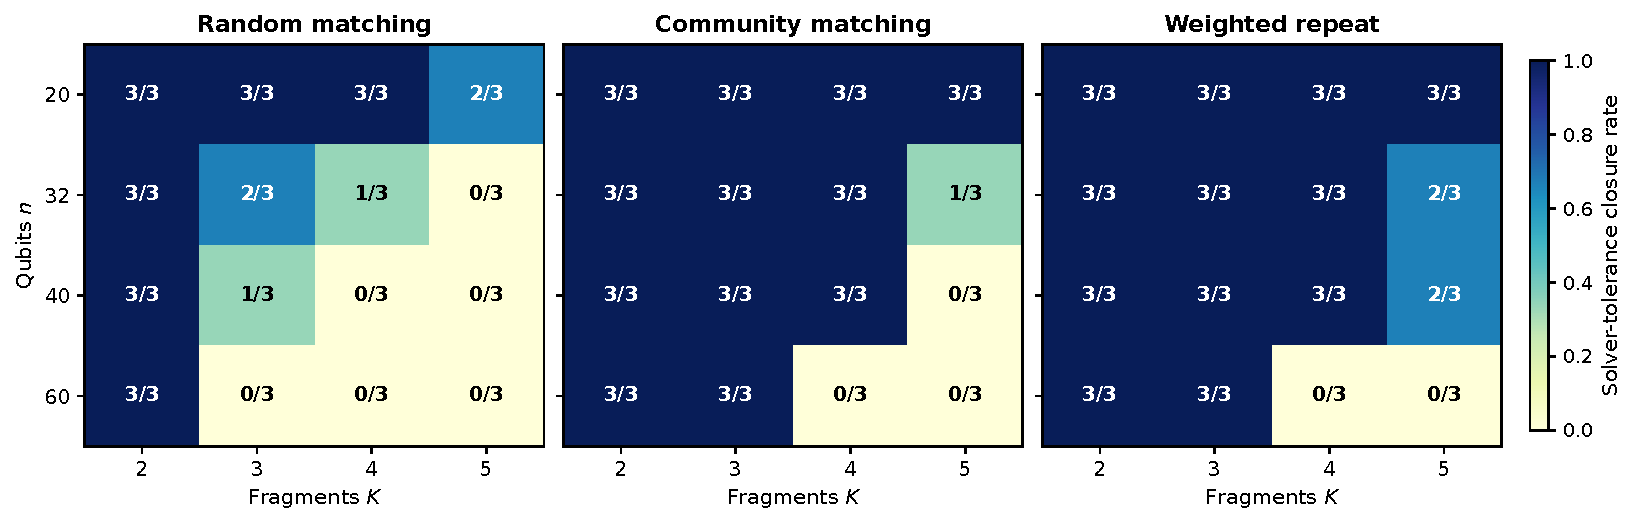
\includegraphics[width=\columnwidth]{fig_e9_closure_heatmap.pdf}
  \caption{E9 solver-tolerance closure counts under a 10-s SCIP limit. Each heatmap cell reports closed runs out of three fixed seeds. The boundary depends materially on graph family, $K$, and seed.}
  \label{fig:e9-closure}
\end{figure}

\begin{figure}[t]
  \centering
  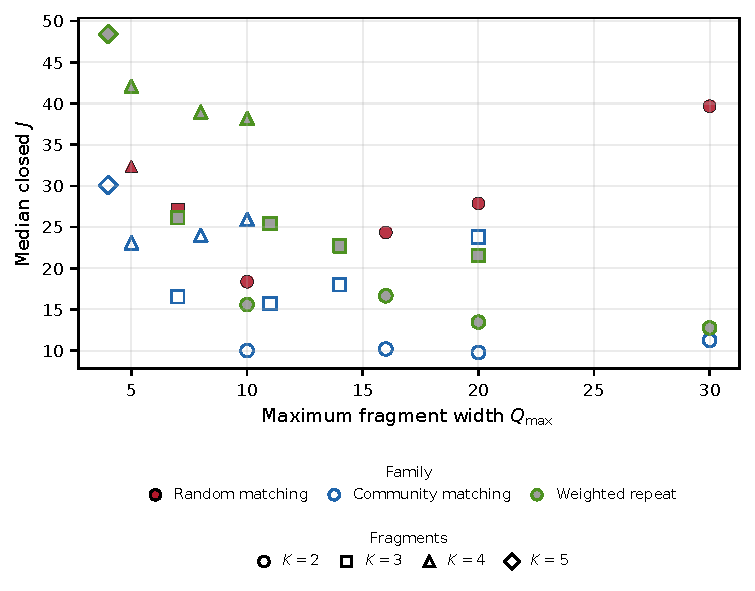
\includegraphics[width=\columnwidth]{fig_e9_width_overhead_pareto.pdf}
\caption{E9 width--overhead tradeoff restricted to cells closed for all three seeds. Colors denote families; markers denote $K$. Each point is the median $\log\Gamma^*$ for its cell. This avoids conditioning the plot on solver-successful seeds.}
  \label{fig:e9-pareto}
\end{figure}

\subsection{Finite-Shot Scope}

Supplementary E8 fixes an equal total ideal-Aer shot budget on three predeclared $n=12$ witnesses. The strong $719.66\times$ modeled reversal reduces RMSE for both observables, whereas a moderate $3.27\times$ reversal is mixed and a no-reversal control is identical under shared seeds. Hence independent-QPD overhead can be operationally informative but is not claimed as a universal finite-shot RMSE predictor. Full witness identities, signed-estimator behavior, and bootstrap intervals remain in the artifact supplement.

\subsection{Artifact Availability}
The accompanying review package contains the reference implementation, frozen raw results, experiment scripts, and SHA-256 manifests. It includes complete E1/E5/E7 generators, deterministic H2 ordering and swap rules, B2S cut policy/tolerance, branching rules, solver options, E6 gate-occurrence accounting, and frozen E8 plan and seed records. For the core K-way evidence it additionally includes the E9 generator, exact near-balanced capacity vectors, fixed gate-cost assignment order, all 144 raw records, the capacity-exact greedy-swap baseline with its restart/seed policy and 144 regret records, the E10 MQT ingestion runner, all 36 valid E10 records, and the three recorded unsupported-VQE ingestion failures.

\subsection{Cardinality and Metrics Are Complementary}

To isolate the source of root-bound strength, we compare four relaxations with identical complete-pair variables and the same LP backend: CP0; CP0 plus cardinality (C); CP0 plus separated metric inequalities (T); and their combination (CT). The study contains 24 circuit-derived instances from the random, dense, weighted-random, and noisy-community families at $n\in\{16,24\}$, with three seeds per cell. C and T each reproduce the CP0 bound on every instance. Proposition~4 explains the CP0+T equality structurally. CT improves all 24 bounds and closes 12 roots, showing empirically that cardinality activates the metric system strongly on this corpus by supplying global cut mass that the metric geometry must distribute.

\begin{table}[t]
\centering
\caption{Root-relaxation decomposition on 24 circuit-derived instances. C and T separately match CP0 on every instance; CT denotes their combination. Gaps are in log-overhead units.}
\label{tab:root-decomposition}
\begin{tabular}{lrrrr}
\toprule
\textbf{Root formulation} & \textbf{Exact} & \textbf{Med. gap} & \textbf{p90 gap} & \textbf{Med. time}\\
\midrule
CP0 & 0/24 & 26.2935 & 52.4468 & 0.3211 s\\
CP0 + C & 0/24 & 26.2935 & 52.4468 & 0.3429 s\\
CP0 + T & 0/24 & 26.2935 & 52.4468 & 0.2832 s\\
CP0 + C + T & 12/24 & 0.2848 & 3.8761 & 2.3222 s\\
\bottomrule
\end{tabular}
\end{table}

Separating all violated triangles at $n\in\{32,40\}$ exceeded the 10-min audit budget before a complete matrix was obtained; we therefore report no tail result for this study.

\subsection{Strengthening Improves Reference-Search Closure}

Table~\ref{tab:ablation} reports a controlled 90-instance ablation with a common 100-node budget. A0 closes 41 gaps, regardless of whether H2 is enabled. Both B2S-root configurations close all 90 with a median of one explored node. Within this protocol, the complete-pair strengthening, rather than incumbent construction, explains the change. Because A0 and B2S use different pair spaces, this ablation measures the package rather than only C and T; Table~\ref{tab:root-decomposition} provides the matched-representation isolation. The SCIP audit above further shows that neither result establishes general solver superiority.

\begin{table}[t]
\centering
\caption{Controlled ablation on 90 synthetic balanced instances under a 100-node budget. ``Closed'' means solver-tolerance gap at most $10^{-9}$; node-limited runs may also be closed.}
\label{tab:ablation}
\resizebox{\columnwidth}{!}{%
\begin{tabular}{lcccc}
\toprule
\textbf{Configuration} & \textbf{Closed} & \textbf{Node-lim.} & \textbf{Med. nodes} & \textbf{Root / Tree (s)}\\
\midrule
A0 + H0 (basic)   & 41/90 & 56 & 100 & 0.000\,/\,2.059\\
A0 + H2            & 41/90 & 52 & 100 & 0.000\,/\,2.072\\
B2S-root + H0       & 90/90 &  0 &   1 & 0.260\,/\,0.060\\
B2S-root + H2       & 90/90 &  0 &   1 & 0.256\,/\,0.063\\
\bottomrule
\end{tabular}
}
\end{table}

\subsection{Legacy Reference Scope}

The artifact supplement retains E1, the 420-instance CNOT-only characterization of the $K=2$ B2S reference implementation. E7 is the matched production-backend result: basic SCIP closes 200/200 heterogeneous $K=2$ records within 10~s and outperforms the specialized reference. We therefore use the legacy material only to document B2S polyhedral behavior, not as a central K-way scalability claim.

\subsection{Representation Sensitivity}

We compare paired representations of identical MQT~Bench source circuits, binding QAOA~\cite{farhi2014} parameters to $\pi/4$. One representation uses the CX-normalized basis $\{RZ,SX,X,CX\}$; the other preserves supported native two-qubit gates. For QAOA at $n=16$, the native $RZZ$ circuit contains 114 two-qubit gates rather than 228 and reduces the optimum from $J^*_{\mathrm{CX}}=158.200$ to $J^*_{\mathrm{native}}=79.100$. Exponentiating the difference gives a modeled overhead ratio of $2.25\times10^{34}$. Bernstein--Vazirani (BV) and VQE~\cite{peruzzo2014,mcclean2016} provide negative controls: their paired $CZ$ or $CX$ representations yield ratio one.

These ratios compare representation-dependent independent-QPD objectives under Qiskit Addon Cutting~0.10. They do not imply an intrinsic reduction in the physical shot complexity of the underlying algorithms.

\begin{table}[t]
\centering
\caption{Optimal objectives under paired CX-normalized and native representations. QAOA is representation-sensitive; BV and VQE are ratio-one controls.}
\label{tab:native}
\resizebox{\columnwidth}{!}{%
\begin{tabular}{llcccc}
\toprule
\textbf{Family} & $\boldsymbol{n}$ & \textbf{CX 2q} & \textbf{Native 2q} & $\boldsymbol{J^*_{\mathrm{CX}}}$ & $\boldsymbol{J^*_{\mathrm{native}}}$\\
\midrule
QAOA & 8  &  56 &  28 &  52.733 & 26.367\\
QAOA & 12 & 144 &  72 & 114.256 & 57.128\\
QAOA & 16 & 228 & 114 & 158.200 & 79.100\\
BV   & 8/12/16 & 3/5/7 & 3/5/7 & 0 & 0\\
VQE  & 8/12/16 & 21/33/45 & 21/33/45 & 6.592 & 6.592\\
\bottomrule
\end{tabular}
}
\end{table}

\begin{figure}[t]
  \centering
  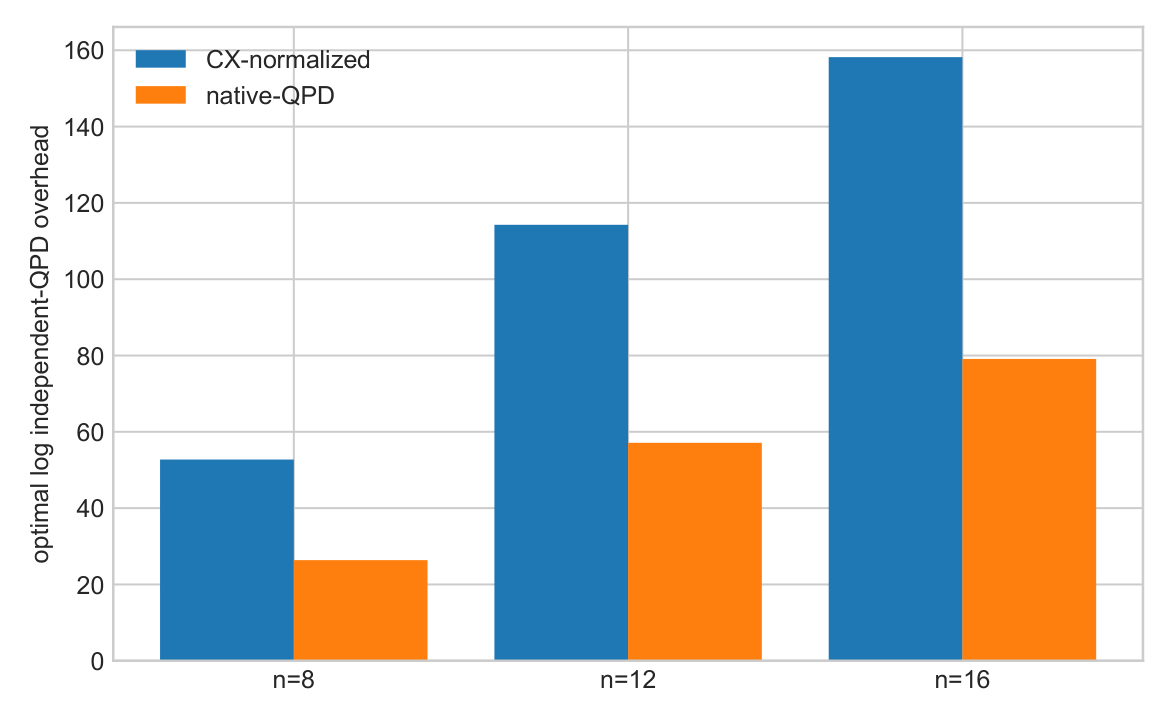
\includegraphics[width=\columnwidth]{fig_native_qaoa_representation.png}
  \caption{QAOA representation sensitivity under the independent-QPD model. Native $RZZ$ circuits contain fewer two-qubit gates and incur a smaller modeled optimum than their CX-normalized counterparts.}
  \label{fig:native}
\end{figure}

\subsection{Comparison with Practical Automatic Cutting}

E4 contains 60 Qiskit cut-finder records for QAOA, BV, and VQE at $n\in\{8,12,16\}$. Qiskit marks 24 records as ``minimum reached.'' For these records, the best balanced-$K=2$ objective equals the reported practical objective within numerical tolerance: the median, 90th percentile, and maximum restriction factors are 1.0, 1.0, and $1.000000000000007$. The agreement includes BV cases where Qiskit returns more than two fragments.

This is a narrow overlap result, not evidence of equivalence between balanced bisection and unconstrained practical cutting. It covers three circuit families, three sizes, one QPD model, and only records carrying Qiskit's own optimality flag.

\subsection{Exact Reconstruction Sanity Checks}

We pass two selected partitions through Qiskit's complete gate-cutting pipeline: QPD replacement, fragment-experiment generation, exact statevector evaluation of every subexperiment, and observable reconstruction. For a six-qubit QAOA circuit, two native $RZZ$ cuts give predicted and executed overhead $\Gamma=33.9706$ and absolute reconstruction error $1.39\times10^{-17}$. For a six-qubit VQE circuit, one CX cut gives overhead 9 and error $5.55\times10^{-17}$. In both cases, the reconstructed expectation agrees with the uncut statevector to machine precision.

This small-scale test checks cost accounting and pipeline compatibility. It does not evaluate finite-shot variance: every QPD basis term is evaluated exactly. Supplementary E8 supplies the separate finite-shot sanity study.

\begin{table}[t]
\centering
\caption{Exact reconstruction check. Predicted and Qiskit-derived overheads agree; ``Abs. error'' compares reconstructed and uncut observables.}
\label{tab:operational}
\resizebox{\columnwidth}{!}{%
\begin{tabular}{lcccc}
\toprule
\textbf{Circuit} & \textbf{Cuts} & \textbf{Pred. $\Gamma$} & \textbf{Exec. $\Gamma$} & \textbf{Abs. error}\\
\midrule
QAOA $n\!=\!6$, native $RZZ$ & 2 & 33.9706 & 33.9706 & $1.39\!\times\!10^{-17}$\\
VQE $n\!=\!6$, CX             & 1 & 9       & 9       & $5.55\!\times\!10^{-17}$\\
\bottomrule
\end{tabular}
}
\end{table}

% ===================================================================
% VI. RELATED WORK
% ===================================================================
\section{Related Work}

Peng et al.~\cite{peng2020} introduced circuit cutting for evaluating circuits wider than the available quantum device, building on quasiprobability simulation~\cite{bravyi2016}. Mitarai and Fujii developed virtual-gate constructions and overhead bounds for nonlocal channel simulation~\cite{mitarai2021,mitarai2021overhead}. Harrow and Lowe characterize cut costs through product extent and give cost bounds for spacelike and timelike cuts~\cite{harrowlowe2025}. CutQC couples automatic partitioning with classical recombination~\cite{tang2021}, while Qiskit Addon Cutting implements gate-level QPD experiment generation and reconstruction~\cite{qiskitcutting}. Complementary directions include maximum-likelihood fragment tomography~\cite{perlin2021}, fragmentation for error reduction~\cite{fragqc}, operator backpropagation~\cite{pal2026}, and sampling bounds beyond bipartitions~\cite{nakamura2025}.

Nakamura, Satoh, and Sanji~\cite{nakamura2025} study sampling bounds and scalable partitioning beyond bipartitions. Their objective and cut-placement setting address multi-fragment cutting directly. \CertiCut{} instead fixes an independent gate-QPD registry and solves a capacitated graph-partitioning MIP, translating a valid global log-objective gap into a multiplicative model-overhead factor. Fr{\"o}hler et al.~\cite{frohler2026} propose a broader scalable heuristic framework for combined gate cuts, wire cuts, and joint gate groups. Their cut-mechanism scope is broader; \CertiCut{} is narrower and focuses on the fixed independent-QPD objective and solver-tolerance global-bound semantics.

Brandhofer, Polian, and Krsulich~\cite{brandhofer2024} optimize richer circuit-knitting partitions that jointly select gate and wire cuts, ancilla insertions, and classical communication under gate-dependent execution and sampling costs. Idan et al.~\cite{idan2026} establish NP-completeness for general cut placement and use SMT for bounded-size fragments. These works are broader along the axis of cut mechanics and execution resources. \CertiCut{} generalizes its earlier bisection formulation along different axes: declared fragment count, capacity constraints, and translation of a global independent-QPD optimization gap into a multiplicative model-overhead factor. In distributed quantum computing, multilevel temporal-hypergraph partitioning instead optimizes teleportation and entanglement cost~\cite{burt2026}; it is a distinct resource model from circuit cutting.

\CertiCut{} deliberately fixes a per-gate independent-QPD registry, then optimizes capacitated $K$-way placement of those costs across a partition. Weighted graph partitioning, branch-and-bound bounds, fixed-capacity cardinality, and metric inequalities are established optimization machinery~\cite{deza1997,lawler1966}; we do not claim them as new. Our contribution is the model specialization and its resource-interpretable bound semantics, controlled and algorithm-derived objective-reversal evidence, and transparent backend evaluation. E7 does not claim a specialized branch-and-bound procedure dominates general-purpose optimization; it shows the opposite on the evaluated $K=2$ corpus. Rather, the exact model reduction and factor semantics are directly usable by a mature optimizer. Multilevel partitioners such as KaHIP~\cite{kahip} provide strong feasible bisections but do not supply the same global bound.

Supplementary E8 does not establish globally optimal decomposition cost. It tests only whether plan differences under the specified independent-QPD objective can have finite-shot consequences in the evaluated ideal-simulator implementation.

% ===================================================================
% VII. LIMITATIONS AND CONCLUSION
% ===================================================================
\section{Limitations and Conclusion}

\subsection{Limitations}

The core formulation is restricted to gate-cut partitions under a fixed circuit representation, logical interaction graph, and independent per-gate QPD registry. It supports arbitrary declared $K$ and capacity bounds but does not optimize wire cuts, exact global routing, hardware noise, or an end-to-end physical execution objective. Joint QPD can reduce sampling overhead when compatible cut gates admit a collective decomposition, but its structural cost semantics lie outside the independent per-gate model optimized here; general joint-aware partition optimization remains future work~\cite{schmitt2025}. The sparse K-way LP relaxation is weak; the tested dense cardinality/metric extension improves neither closure nor runtime at the reported scale. E9 uses three deterministic seeds per family--size--$K$ cell; this replication exposes seed sensitivity but remains a fixed matrix rather than a workload-prevalence estimate. Random-matching $K\geq3$ instances retain weak factors at 10~s. E10 broadens the evidence to a small algorithm-derived matrix but remains non-prevalence evidence. Supplementary E8 evaluates finite-shot behavior rather than modeling it. Finally, empirical optimization bounds are obtained from floating-point solvers. They are solver-tolerance quantities and have not been independently verified using directed rounding, rational reconstruction, or another rigorous lower-bound procedure.

The frozen manifest records software versions, solver tolerance, seeds, experiment counts, and SHA-256 hashes. Reproducing the reported numbers requires this protocol; changing the solver stack requires regenerating the evidence.

\subsection{Conclusion}

For capacitated $K$-way gate partitioning under a fixed independent per-gate QPD model, we showed that the log-overhead objective reduces exactly to weighted graph partitioning. This reduction gives a backend-independent interpretation of optimization uncertainty: in exact arithmetic, any global primal/lower-bound pair $(\UB,\LB)$ bounds incumbent model overhead by $\exp(\UB-\LB)$. Controlled and algorithm-derived experiments show that minimizing cut count can select partitions with substantially larger independent-QPD overhead.

The solver studies establish three results. On the frozen 200-instance $K=2$ E7 corpus, basic SCIP is substantially stronger than the specialized \CertiCut{} reference implementation, closing 200/200 instances within 10~s. On replicated E9, SCIP closes 101/144 heterogeneous $K$-way runs through $n=60$ and reports explicit factors for every open case. The capacity-exact weighted K-way baseline returns all 144 feasible plans in milliseconds; SCIP bounds show its median regret factor is 28.05 on closed records. E10 reproduces a nontrivial K-way boundary on algorithm-derived circuits. We therefore make no custom-solver superiority or universal large-$K$ scalability claim; \CertiCut{} is a formulation, semantic reporting layer, and reproducible reference implementation that can use mature MIP engines.

The equal-total-shot E8 study provides conditional operational evidence. Verified numerical bounds, broader E9 workload coverage, and broader finite-shot workloads remain future work.

% ===================================================================
\section*{Acknowledgment}
The authors gratefully acknowledge the open-source communities behind Qiskit, Qiskit Addon Cutting, SciPy/HiGHS, KaHIP, and MQT~Bench, whose software made the implementation and evaluation of this work possible.

% ===================================================================
% APPENDICES
% ===================================================================
\appendices

\section{Family-Level Results at $n = 40$}
\label{app:n40}

Table~\ref{tab:n40} breaks down the largest evaluated size by graph family. Median time ranges from 0.809~s for community instances to 37.215~s for weighted-random instances. These values describe the evaluated samples; they do not establish a causal relationship between graph structure and computational difficulty.

\begin{table}[h]
\centering
\caption{Family-level performance breakdown at $n = 40$. Each family contains ten seeded instances.}
\label{tab:n40}
\resizebox{\columnwidth}{!}{%
\begin{tabular}{lccc}
\toprule
\textbf{Family} & \textbf{Solver-tol. closed} & \textbf{Med. time (s)} & \textbf{p90 time (s)}\\
\midrule
Community        & 10/10 &  0.809 &  1.186\\
Nearest-neighbor & 10/10 &  1.646 &  1.764\\
QAOA ring        & 10/10 &  5.367 &  6.173\\
Noisy-community  &  9/10 &  2.419 & 18.188\\
Random           & 10/10 & 18.344 & 41.224\\
Dense            & 10/10 & 24.070 & 52.669\\
Weighted-random  &  8/10 & 37.215 & 60.067\\
\bottomrule
\end{tabular}
}
\end{table}

\section{Bound-Report Semantics}
\label{app:cert}

We evaluate $F$ in the log domain to avoid overflow. ``Closed'' means a solver-reported gap $\UB-\LB\leq10^{-9}$; it is not an independently verified exact proof. ``Bound report unavailable'' means that no safe boundary has completed by the checkpoint. At 60~s, all E1 runs have finite bounds; the three open runs retain positive gaps and nonempty frontiers and are classified as time-limit bound reports.

\bibliographystyle{IEEEtran}
\bibliography{references}

\end{document}
